% oja_template.tex
% Unofficial LaTeX template for publishing 
% in the Open Journal of Astrophysics
% v1.0 released September 6, 2015 (matches openjournal.cls)
% Author: Emmanuel Frion

% Basic setup
\documentclass[twocolumn]{openjournal}
% Available options:
% [twocolumn] - two-column mode
% [onecolumn] - (default) main text in one-column mode
% [apj]       - typeset in the style of ApJ.
% [apjl]      - (default) typeset in the style of ApJ Letters 
% [tighten]   - some adjustments to approximate grid typesetting
% [numberedappendix]   - number appendix sections as A, B, etc
% [appendixfloats]  - use separate numbering for floats within appendix
% [twocolappendix]  - make appendix in two-col mode in a two-col paper
% [revtex4]   - force using revtex4 (rather than 4-1)

% Remove this package
\usepackage{lipsum}

% In case of issues with doi formatting, uncomment these lines
% \let\olddoi\doi
% \renewcommand{\doi}[1]{\href{https://doi.org/#1}{DOI: \nolinkurl{#1}}}

% Optional useful packages
\usepackage{xcolor}
\usepackage{textgreek}
\usepackage{tikz}
\usepackage[utf8]{inputenc}
\usepackage[english]{babel}

\usepackage{hyperref}
\hypersetup{
    unicode, 
    colorlinks=true,
    linkcolor=linkcolor,
    citecolor=linkcolor,
    filecolor=linkcolor,
    urlcolor=linkcolor,
}
\usepackage{color,colortbl}
\definecolor{linkcolor}{rgb}{0.0,0.3,0.5}
\usepackage{tensind}
\tensordelimiter{?}
\DeclareGraphicsExtensions{.bmp,.png,.jpg,.pdf}
\usepackage{verbatim}
\usepackage[normalem]{ulem}
\usepackage{orcidlink}
\usepackage{soul}

\urlstyle{same}

% Define path to put your plots, figures, etc...
\graphicspath{ {./figs/} }


\usepackage{newtxtext,newtxmath}
% Depending on your LaTeX fonts installation, you might get better results with one of these:
%\usepackage{mathptmx}
%\usepackage{txfonts}

% Use vector fonts, so it zooms properly in on-screen viewing software
% Don't change these lines unless you know what you are doing
\usepackage[T1]{fontenc}
% \usepackage{amsmath, graphicx, dcolumn, color, units,  mathtools, physics, tensor, bm, lipsum, revsymb}

% Only include extra packages if you really need them. Common packages are:
\usepackage{graphicx}	% Including figure files
\usepackage{amsmath, amssymb, graphicx, color, units}
% \usepackage{amsmath}	% Advanced maths commands
% \usepackage{amssymb}	% Extra maths symbols

% \usepackage{xspace}
% \newcommand{\GpcminThree}{\ensuremath{\,\rm{Gpc}^{-3}}\xspace}
% \newcommand{\yearmin}{\ensuremath{\,\rm{yr}^{-1}}\xspace}
% units 


\usepackage{acro}

\DeclareAcronym{ZAMS}{
  short = ZAMS ,
  long  = zero-age main sequence
}



\newcommand{\Rsun}{\ensuremath{\,\rm{R}_{\odot}}\xspace}
\newcommand{\km}{\ensuremath{\,\rm{km}}\xspace}
\newcommand{\kms}{\ensuremath{\,\rm{km}\,\rm{s}^{-1}}\xspace}
\newcommand{\Msun}{\ensuremath{\,\rm{M}_{\odot}}\xspace}
\newcommand{\Lsun}{\ensuremath{\,\rm{L}_{\odot}}\xspace}
\newcommand{\kpc}{\ensuremath{\,\rm{kpc}}\xspace}
\newcommand{\Mpc}{\ensuremath{\,\rm{Mpc}}\xspace}
\newcommand{\Zsun}{\ensuremath{\,\rm{Z}_{\odot}}\xspace}
\newcommand{\AU}{\ensuremath{\,\mathrm{AU}}\xspace}
\newcommand{\Myr}{\ensuremath{\,\mathrm{Myr}}\xspace}
\newcommand{\yr}{\ensuremath{\,\mathrm{yr}}\xspace}
\newcommand{\yrs}{\ensuremath{\,\mathrm{yr}}\xspace}
\newcommand{\Myrs}{\ensuremath{\,\mathrm{Myr}}\xspace}
\newcommand{\Gyr}{\ensuremath{\,\mathrm{Gyr}}\xspace}
\newcommand{\Gyrs}{\ensuremath{\,\mathrm{Gyr}}\xspace}
\newcommand{\Kelvin}{\ensuremath{\,\mathrm{K}}\xspace}
\newcommand{\yearmin}{\ensuremath{\,\rm{yr}^{-1}}\xspace}
\newcommand{\MpcminThree}{\ensuremath{\,\rm{Mpc}^{-3}}\xspace}
\newcommand{\GpcminThree}{\ensuremath{\,\rm{Gpc}^{-3}}\xspace}

\usepackage[table]{xcolor}
\usepackage{colortbl}


%% MODELS 

\newcommand{\CfA}{Center for Astrophysics \textbar{} Harvard $\&$ Smithsonian,
60 Garden St., Cambridge, MA 02138, USA}

\newcommand{\SoF}{Simons Society of Fellows, Simons Foundation, New York, NY 10010, USA}
\newcommand{\Columbia}{Department of Astronomy, Columbia University, 538 West 120th Street, New York, NY 10027, USA}
\newcommand{\JHU}{William H. Miller III Department of Physics and Astronomy, Johns Hopkins University, Baltimore, Maryland 21218, USA}
\newcommand{\AstroAI}{AstroAI at the Center for Astrophysics \textbar{} Harvard \& Smithsonian, 60 Garden St., Cambridge, MA 02138, USA}
\newcommand{\CUNY}{Graduate Center, City University of New York, 365 5th Avenue, New York, NY 10016, USA}
\newcommand{\UCSD}{Department of Astronomy and Astrophysics, University of California, San Diego, La Jolla, CA 92093, USA}
\newcommand{\CAMK}{Nicolaus Copernicus Astronomical Center, Polish Academy of Sciences, ul. Bartycka 18, 00-716 Warsaw, Poland}


\begin{document}


\title{Software Citation Cookbook/Primer }

% \author{Floor S. Broekgaarden\orcidlink{0000-0002-4421-4962}}
% \email{fbroekgaarden@ucsd.edu}
% \affiliation{\UCSD}



\author{ET AL  \orcidlink{0000-0000-0000-0000}}
\email{author2@you.com}



\begin{abstract}
\textbf{make a google docs to help with people are a bit shy }
\end{abstract}

% Write your keywords here
\begin{keywords}
    {First, second}
\end{keywords}


\maketitle



% These are old, but perhaps useful still:

% N. P. Chue Hong, A. Allen, A. Gonzalez-Beltran, A. de Waard, A. M. Smith, C. Robinson, C. Jones, D. Bouquin, D. S. Katz, D. Kennedy, G. Ryder, J. Hausman, L. Hwang, M. B. Jones, M. Harrison, M. Crosas, M. Wu, P. Löwe, R. Haines, S. Edmunds, S. Stall, S. Swaminathan, S. Druskat, T. Crick, T. Morrell, T. Pollard, “Software Citation Checklist for Authors,” Zenodo, 15-Oct-2019. https://doi.org/10.5281/zenodo.3479198
% N. P. Chue Hong, A. Allen, A. Gonzalez-Beltran, A. de Waard, A. M. Smith, C. Robinson, C. Jones, D. Bouquin, D. S. Katz, D. Kennedy, G. Ryder, J. Hausman, L. Hwang, M. B. Jones, M. Harrison, M. Crosas, M. Wu, P. Löwe, R. Haines, S. Edmunds, S. Stall, S. Swaminathan, S. Druskat, T. Crick, T. Morrell, T. Pollard, “Software Citation Checklist for Developers,” Zenodo, 15-Oct-2019. https://doi.org/10.5281/zenodo.3482768
% From https://github.com/force11/force11-sciwg






% \begin{table}[h!]
% \centering
% \renewcommand{\arraystretch}{1.5}

% \begin{tabular}{|c|c|c|c|c|c|c|}
% \hline
% \cellcolor{red!30}\makebox[0.2\linewidth]{1} &
% \cellcolor{orange!40}\makebox[0.2\linewidth]{2} &
% \cellcolor{yellow!50}\makebox[0.2\linewidth]{3} &
% \cellcolor{green!30}\makebox[0.2\linewidth]{4} &
% \cellcolor{cyan!30}\makebox[0.2\linewidth]{5} &
% \cellcolor{blue!25}\makebox[0.2\linewidth]{6} &
% \cellcolor{violet!30}\makebox[0.2\linewidth]{7} \\
% \hline
% & & {\multicolumn{4}{|c|}{SCS}} & \\
% \hline 
%  & & \multicolumn{2}{|c|}{ASCL} & & & \\
% \hline
%  & & & & & & \\
% \hline
%  & & & & & & \\
% \hline
% \end{tabular}


% \vspace{3cm}

% \caption{Top row fully colored per cell}
% \end{table}

\section{A Primer on Software Citation in Astronomy}
based on:
\url{https://zenodo.org/records/3482769}
\url{https://elib.dlr.de/133078/1/software_citation_checklist_for_authors.pdf} (Are these the same) 
\subsection*{Why software citation matters}
\begin{itemize}
    \item Software is now foundational to nearly all areas of astronomy, enabling data processing, simulations, and analysis pipelines.
    \item Proper citation ensures credit, reproducibility, and long-term sustainability of scientific software.
    \item Despite its importance, software is often inconsistently cited due to lack of standardization and discoverability of references.
\end{itemize}

\begin{figure*}
  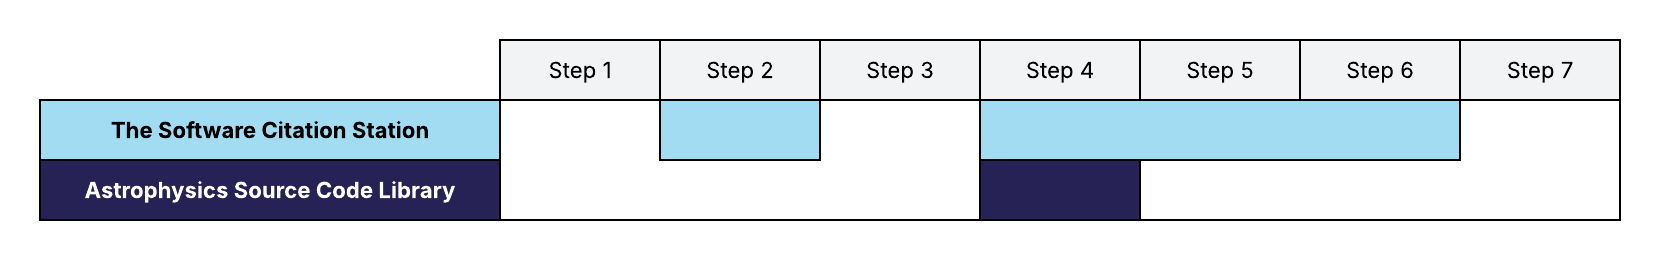
\includegraphics[width=\textwidth]{figs/citation_tools.png}

\end{figure*}


\subsection*{Part I: How to cite software in your research}

\begin{enumerate}
    \item \textbf{Inventory your software} \\
    Go through your analysis scripts, notebooks, and pipelines to identify all software used (both direct and indirect). 
What should you include? (decision tree) 
\begin{itemize}
    \item is it citeable? %URLs are not citeable, does it have a DOI or some other persistant identifier (PID)? 
    \item do they need the credit/citation? 
    \item will it make your work easier to reproduce? 
    \item do you feel you should give credit? 
\end{itemize}
\textbf{refer to oappendix for nuance}

\item \textbf{Consider dependencies} \\
    Many tools rely on other packages which represent real intellectual contributions. If you feel that these dependencies are important to your research using the above metrics, even if you do not use them directly, they should also be cited. See \S\ref{ap:ap} for further discussion on this topic.


  \item \textbf{Figure out software versions} \\
    Note the version numbers of each package used. Software evolves rapidly, and reproducibility requires version-specific attribution. You can run the following commands to list all installed packages and their versions. 

\begin{verbatim}
pip list
conda list
--version
\end{verbatim}

    \item \textbf{Check recommended citations for each package} \\
    Many software packages provide explicit citation instructions (e.g., in documentation, README, or CITATION.cff files). Follow these exactly when possible.

    % \item \textbf{Include non-traditional resources} \\
    % Consider citing databases (e.g., ADS), analysis tools, or web-based platforms that contributed to your results.

    % \item \textbf{Use tools to streamline citation collection} \\
    % Tools such as the \textit{Software Citation Station} can automatically generate acknowledgements and BibTeX entries based on selected software and versions.


    \item \textbf{Compile/Create BibTeX entries in your bibliography for each software entry} \\

    \texttt{@software} or \texttt{@misc}
    % how to do it yourself 
    % Ensure all cited software has corresponding entries in your reference list, preferably with persistent identifiers (e.g., DOI).

    % \item \textbf{Check journal-specific policies} \\
    % Some journals (e.g., AAS journals) have dedicated software sections or formatting requirements—adapt your citations accordingly.
    

    \item \textbf{Add a Software Acknowledgement section in your paper} \\
    Combine software acknowledgements into a coherent paragraph (often placed in the acknowledgements or a dedicated software section). Check your journal for specific software acknowledgement. \\
    
    \textit{examples }\\



    \item \textbf{Perform a final check} \\
    Ask: is all relevant software acknowledged? 
    could another researcher reconstruct your computational setup from your citations alone? If not, refine. Does everything have ? 
    \textbf{NO URLs}
\end{enumerate}

\section*{Part II: How to make your software citable (checklist)}

% In rough order of importance: 
% - get a doi! Either by for a related paper or directly for your software. 
% - clearly list your preferred citation 
% - maintain and update
% - include version control 
% - consider adding to a community resource
% - document well 


what is citeable;
get credit in a paper, following today's citation practices/journal; 
get a doi

\begin{enumerate}
%     \item \textbf{Publish your software in a public repository} \\
%     Host your code on a public platform (e.g., GitHub) with clear documentation, version control and licensing information.


% \href{https://onegoodtutorial.org/in-depth/software-citation/}{The One Good Tutorial Software Citation Guide}.

%     \item \textbf{Document dependencies and metadata} \\
%     Clearly list dependencies, programming language, and scientific domain to facilitate proper attribution and reuse. 
% \begin{verbatim}
% Requirements.txt (python)\\
% pip requirements 
% \end{verbatim}
    


    \item \textbf{Get a persistent, versioned, identifier (DOI)} \\
    Use services such as Zenodo/Figshare to create  DOIs that allow precise citation of releases. Zenodo and similar resources also support version control. RRID if its not public. Note that GitHub has a collaboration with Zenodo that allows you to automatically submit it to Zenodo and connect it 


        \item \textbf{Provide citation instructions} \\
    Can be done multiple ways; e.g.
    (Preferred) Include a \texttt{CITATION.cff} \texttt{CodeMeta} file or (less preferred) a dedicated section in your README specifying how your software should be cited. 
    \textit{Examples: }
    \url{https://citation-file-format.github.io/}

    
    \item \textbf{Maintain and update citation information} \\
    As your software evolves, keep citation instructions and metadata up to date to reflect new versions and contributions.
    \textbf{see TARDIS example}

    % \item \textbf{Support versioned citation} \\
    % Ensure users can cite specific versions of your code, as results may depend on implementation details. 
\end{enumerate}

    \section*{Optional: make it more ctieable}
    \begin{itemize}

    \item \textbf{Add your software to community resources?} \\
    Submit your code to resources such as ASCL, or the Software Citation Station so that it might be easier to find your citation/software. %or similar registries to improve discoverability and standardization.

    \item \textbf{Consider publishing a software paper} \\
    Journals such as JOSS provide peer-reviewed publications for software, which can serve as a canonical citation. There are also other journals like ApJS (\textbf{other examples} ) that encourage software-focused publications. (e.g. through living documents). 


    \item \textbf{Highlight your software impact}
    we recommend on your CV to highlight number of citations, software mentions (ADS), zenodo downloads. 
    Examples can be found here 
    use of affiliated 
    Github forks, stars, 
    analytics trackers,
    number of forward/upstream dependencies,
    %

    % \item \textbf{Encourage citation in your community} \\
    % Explicitly remind users (in documentation and talks) to cite your software and explain why it matters.

    \end{itemize}






\section{Appendix: On What (and How Much) to Cite}

There is no single, universally agreed-upon answer to what software should be cited, nor to how extensively one should cite software dependencies. This ambiguity is not unique to software: it closely mirrors the broader challenge in scholarly writing of deciding which prior works merit citation in the main body of a manuscript. In both cases, citation practices involve judgment rather than strict rules.


In practice, authors must make informed, context-dependent decisions. A useful guiding principle is to cite with care: consider whether a piece of software made a meaningful intellectual or practical contribution to your work, whether it is citable (e.g., has a DOI or recommended/preferred citation), and whether providing a citation meaningfully contributes to reproducibility or credit. In some cases, citations can directly support the individuals and teams behind the software, particularly for community-developed scientific tools, by improving visibility, funding prospects, and career recognition. In other cases (e.g., ubiquitous infrastructure such as programming languages), the marginal benefit of citation may be less clear.

These considerations apply both to which software to cite (e.g., whether to cite high-level tools versus underlying infrastructure) and to whether and how to cite dependencies. Dependencies represent real intellectual contributions, but citing every layer of a software stack is often impractical and may not align with journal norms.

Ultimately, software citation remains an evolving practice, with expectatiions varying across fields, collaborations, and journals. Rather than prescribing a rigid rule, this primer advocates for a thougthtful and intentional approach: be aware of the impact of your choices, aim for transparency and reproducibility, and make a good-faith effort to give appropriate credit where it is due.



\newpage 








\subsection{Part II-prime: How to make your software citable}

\textit{Adapted from \href{https://onegoodtutorial.org/in-depth/software-citation/}{The One Good Tutorial Software Citation Guide}.}

\subsubsection{Choose Your Strategy}

To make your software itself citable --- as distinguished from writing a traditional article 
about your software --- you first need to publish it in some fashion. We recommend that you choose one of two main publication strategies.

\subsubsection{Option 1: Zenodo}

The free CERN-supported service \href{https://about.zenodo.org/}{Zenodo} can take care of the nuts and bolts of making software citable: it accepts uploads of arbitrary files (e.g., source code packages), guarantees their long-term preservation, and can mint associated DOIs with proper metadata. Citations of those DOIs are, in as true a way as we have, citations of the software itself.

In order to support multiple releases of the same piece of software, Zenodo supports a concept called \href{https://zenodo.org/help/versioning}{DOI versioning}. To really do a gold-standard job of publishing citable software, you ought to understand how this versioning works and set up some kind of automation to deposit every release of your software with Zenodo. \href{https://docs.github.com/en/repositories/archiving-a-github-repository/referencing-and-citing-content}{GitHub has built-in support for this} that probably meets your needs. If you're not using GitHub or want finer-grained control over things, look into release automation tools such as \href{https://pkgw.github.io/cranko/book/latest/integrations/zenodo.html}{Cranko}.

If you are publishing your software to Zenodo automatically, you need to think about how you will maintain the publication metadata, most importantly the author list for your software.

\subsubsection{Option 2: The Journal of Open Source Software}

The free, open-access \href{https://joss.theoj.org/about}{Journal of Open Source Software} (JOSS) takes a slightly different tack to help make software citable. JOSS is a ``software journal'': it looks and works like any other academic journal, but instead of submitting manuscripts to it, you submit software. Your software is peer-reviewed and, if it passes review, your software gets published. The JOSS team takes on the work of minting a DOI and doing the other tasks to turn your software into a citable object.

People can get a bit confused by JOSS because during its submission process you \textit{do} have to submit a brief manuscript describing the software, and various JOSS pages talk about ``papers'' published in the journal. But at its core, JOSS is about peer-reviewing and publishing \textit{software}, not prose. The associated manuscript PDF is basically an adapter to help JOSS interface with legacy scholarly-publishing workflows (and people) that have trouble understanding that it's possible to cite things that aren't articles.

Note that JOSS therefore doesn't do versioning: they'll only mint a single DOI for your software publication, not a \href{https://zenodo.org/help/versioning}{version DOI} for every release like Zenodo.

\subsubsection{Publish Citation Instructions for Your Software}

With traditional research articles, you have a professional publisher who takes care of telling people how to cite your publication. In the world of software, you're the publisher, so you have to take on that task yourself.

If your software is published to Zenodo, you should direct people to its Zenodo page. The page sidebar includes a ``Citation'' box with the suggested citation text and an ``Export'' box that can be used to export the citation metadata in a variety of common formats.

If your software is published in JOSS, direct people to its JOSS page, which has a comparable ``Citation'' sidebar.

\textit{[Should probably say something about CITATION.cff even though Peter does not believe in it.]}



\subsection{FAQ}

\subsubsection{What if I dont know my version}


\subsubsection{Should I cite word/overleaf etc. (where do we stop)}

\subsubsection{what if there is no DOI} 

\subsection{Take-away message}
\begin{itemize}
    \item Software citation is not an afterthought—it is a core component of modern scientific practice.
    \item Small, consistent efforts by both users and developers can significantly improve credit, reproducibility, and sustainability in astronomy.
    \item Maybe something about new papers that encourage living documents for software publications (like ApJS) 
\end{itemize}


\subsection{A future with AI}
\begin{itemize}
    \item The Software Citation Workshop recognizes that the citation community is in need of a helping hand. is increasingly responding to the expanding role of AI in scholarly and software production. As machine-learning systems become more embedded in the academic workflow, our community is exploring the emerging practices, conceptual frameworks and practice tools to help authors explain the LLM-assisted creation process more clearly and responsibly.
\end{itemize}
\begin{itemize}
    \item This is a developing area rather than a settled standard. The Software Citation Workshop has created tools such as the Model Influence Statement Generator to support structured, voluntary disclosure of model use alongside the established citation and acknowledgment practices. Our aim is to support experimentation, documentation and community-informed refinement instead of impose a one-for-all citation rule. As scholar communication continue to adapt, the Software Citation Workshop welcomes feedback from authors, reviewers, publishers, funders, infrastructure providers and model developers on how these practices should evolve to better support transparency, reproducibility and responsible model use.
\end{itemize}
\section*{Acknowledgments}



\bibliographystyle{apsrev4-1}

% You should give the same name for your .bbl as your main .tex
% since it is a requirement for posting on ArXiv.
\bibliography{oja_template}


\begin{appendix}

\section{Appendix 1}
\label{ap:ap}

Be curious and thoughtful about the software you are using. Try to give credit
where credit is due. Citing is caring
\lipsum[4]

\end{appendix}


 

\end{document}
